% ----------------------------------------------------------
\chapter{Algoritmos e estruturas de dados para consulta de segmentos no plano}
% ----------------------------------------------------------
Nesta seção, veremos formas de construir estruturas de dados que ajudam a responder consultas da seguinte forma: Dado um conjunto de segmentos no plano, quais destes segmentos estão em uma janela? Consideramos que o conjunto de segmentos é fixo. Portanto, uma vez construída, a estrutura de dados estará fixa e preparada para responder muitas consultas diferentes. Veremos duas estruturas de dados neste capítulo: Árvore de Intervalos e Árvore de Segmentos. Para cada estrutura veremos como podemos construí-las e usá-las para responder consultas em janelas.% r os segmentos dentro de uma janela.

% ----------------------------------------------------------
\section{Árvore de Intervalos} \label{interval-tree}
Seja $I$ um conjunto de intervalos. A mediana deste conjunto de intervalos $I$ é a media das medianas de cada intervalo em $I$. Denotaremos que um intervalo $[x, x']$ é menor que $\theta$ se $x' < \theta$. Reciprocamente, denotaremos que o intervalo $[x, x']$ é maior que $\theta$ se $x > \theta$.
Uma árvore de intervalos é uma árvore binária balanceada multinível onde cada nó não folha guarda um valor $v$ que representa a mediana de um conjunto de intervalos $I$. Denotaremos o conjunto de intervalos que contém o valor $v$ de $I_{med}$. Denotaremos também o conjunto de intervalos que são menores que $v$ e não contém $v$ de $I_{esq}$, e similarmente, o conjunto de intervalos maiores que $v$ e que não o contém de $I_{dir}$. Cada nó não folha $r$ possui uma estrutura auxiliar para consultar os intervalos $I_{med}$. Uma árvore de intervalos pode ser construída em tempo $O(n\log(n))$. Uma árvore de intervalos pode reportar todos os $k$ segmentos que estão em uma janela em tempo $O(\log^2(n) + k)$ \cite{cg08}. % onde $k$ é o numero de segmentos para serem reportados. 
A fim de encontrar quais segmentos estão sendo visualizados em uma janela temos três casos. Os segmentos possuem dois pontos dentro da janela; Os segmentos possuem ao menos um dos pontos extremos dentro da janela; Os segmentos possuem nenhum ponto extremo dentro da janela, porem, cruzam a janela. Utilizaremos a árvore de intervalo para encontrar o ultimo caso. Para encontrarmos os dois primeiros utilizaremos as estruturas estudadas na seção \ref{range-tree}.
 
\subsection{Árvore de Intervalos unidimensional}
A construção considera um dado conjunto de intervalos $I$ e pode ser feita da seguinte forma. Temos os intervalos da forma $i = [x,x']$. Ao iniciar a construção, calculamos o valor da mediana, $x_{med}$, dos intervalos em $I$ e o guardamos em um nó $r$. Criamos três subconjuntos $I_{esq}$ e $I_{dir}$ tal que $I_{esq} = \{[x, x'] \in I : x' < x_{med} \}$, $I_{dir} = \{[x, x'] \in I : x > x_{med} \}$ e $I_{med} = \{[x, x'] \in I : x \leq x_{med} \leq x' \}$. Construímos duas estruturas de dados auxiliares $\tau_{esq}(r)$ com todos os intervalos de $I_{med}$ ordenada considerando o ponto mais à esquerda de cada intervalo e $\tau_{dir}(r)$ considerando o ponto mais à direita de cada intervalo. Por fim associamos ambas  $\tau_{esq}(r)$  e  $\tau_{dir}(r)$ ao nó $r$. O processo continua de forma recursiva sobre os dois novos conjuntos $I_{esq}$ e $I_{dir}$. Vamos considerar o seguinte conjunto de intervalos da Figura \ref{fig:18} para ilustrar a construção de uma árvore de intervalos.

\begin{figure}[h!]
    \begin{center}
        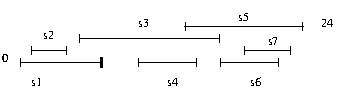
\includegraphics[scale=1.5]{images/interval_tree5.pdf}
    \end{center}
    \caption {— Conjuntos de Intervalos na reta real.}
    \label{fig:18}
\end{figure}

\begin{algorithm}[h!]
    \caption{Recebe um conjunto de intervalos $I$ na reta real. Devolve a raiz de uma árvore de intervalos.}
    \begin{algorithmic}[1]
        \Function{ConstróiÁrvoreDeIntervalos}{$I$}
            \If{$I$ for vazio}
                \Return nó folha vazio
            \Else
                \State Crie um nó $r$
                \State Faça uma ordenação sobre $I$ pelo ponto mais à esquerda
                \State Calcule $x_{med}$ e guarde em $r$ 
                \State Calcule $I_{med}$ construa duas listas ordenadas para $I_{med}$
                \State $\tau_{esq}(r)$ ordenado pelo ponto mais à esquerda dos intervalos crescente
                \State $\tau_{dir}(r)$ ordenado pelo ponto mais à direita dos intervalos decrescente
                \State Guarde $\tau_{esq}(r)$ e $\tau_{dir}(r)$ no nó $r$
                
                \State Cria os nós $r_{esquerda}$ e $r_{direita}$
                \State $r_{esquerda} \leftarrow $ \Call{ConstróiÁrvoreDeIntervalos}{$I_{esq}$}
                \State $r_{direita} \leftarrow $ \Call{ConstróiÁrvoreDeIntervalos}{$I_{dir}$}
                \State Associe $r_{esquerda}$ como filho à esquerda de $r$
                \State Associe $r_{direita}$ como filho à direita de $r$
                \State \Return $r$
            \EndIf
        \EndFunction
    \end{algorithmic}
\end{algorithm}


Vamos seguir alguns passos da construção de uma árvore de intervalos como feito em \cite{cgi1}. Considerando os intervalos da Figura \ref{fig:19} inicialmente vamos ordenar os intervalos de $I$ pelo ponto mais à esquerda: $s_1 = [0, 7]$, $s_2 = [1, 4]$, $s_3 = [5, 12]$, $s_4 = [11,16]$, $s_5 = [14, 24]$, $s_6 = [17, 22]$, $s_7 = [19, 23]$. Criamos um nó raiz $r$ e nele armazenamos o valor da $x_{med}  = 14$. Dividimos o conjunto de intervalos em três subconjuntos: $I_{esq}$ com os segmentos $\{s_1, s_2\}$, $I_{dir}$ com os segmentos $\{s_6, s_7\}$ por fim $I_{med}$ com os segmentos que contêm $x_{med}$ $\{ s_3, s_4, s_5\}$. Com relação a $I_{med}$ construímos duas listas: $\tau_{esq}(r)$ com os intervalos ordenados pelos pontos mais à esquerda $\{s_3,s_4,s_5\}$, e $\tau_{dir}(r)$ com os intervalos ordenados pelos pontos mais à direita de forma decrescente $\{s_5, s_3, s_4\}$. Ordenamos à esquerda de forma crescente nos garantirá que em uma consulta se o valor consultado for menor que o primeiro intervalos consultado, não haverá necessidade de consultar os demais intervalos da lista associada. Respectivamente, os segmentos ordenados de forma decrescente pelos pontos extremos à direita nos garante que caso a consulta seja maior que o primeiro valor da lista não haverá necessidade de continuar a consulta na lista associada à direita. A subárvore à esquerda será uma árvore de intervalos sobre $I_{esq}$; e a subárvore à direita será uma árvore de intervalos sobre $I_{dir}$. Este procedimento é repetido até que o conjunto de intervalos seja vazio. Neste caso, criamos um nó folha também vazio.
A Figura \ref{fig:19} ilustra a árvore de intervalos construída.

\begin{figure}[h!]
    \begin{center}
        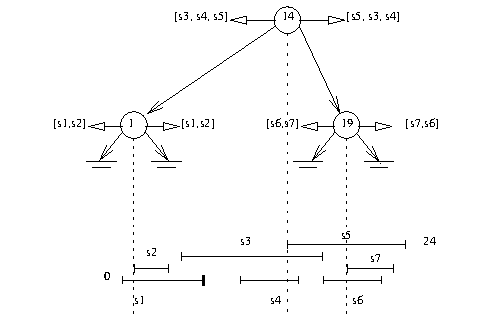
\includegraphics[scale=1.5]{images/interval_tree1.pdf}
    \end{center}
    \caption {— Árvore de Intervalos.}
    \label{fig:19}
\end{figure}

\subsection{Consulta de ponto em árvores de intervalo}
Seja uma árvore binária de intervalos $T$. Uma consulta nesta árvore é tal que queremos todos os intervalos que contenham o valor $q_x$ consultado. Dado o valor $q_x$ da consulta realizamos o seguinte algoritmo: inicialmente checamos se $q_x$ é menor que o valor armazenado em $r$ (denotaremos por $q_x < r$); Caso seja, consultaremos a lista auxiliar $\tau_{esq}(r)$ e retornamos todos os intervalos que contenham $q_x$; então fazemos recursivamente a consulta em $r_{esquerda}$. De forma simétrica, caso $q_x \geq r $  consultaremos a lista auxiliar $\tau_{dir}(r)$ retornando os intervalos que contenham $q_x$ e recursivamente consultando em $r_{direita}$.

\begin{figure}[h!]
    \begin{center}
        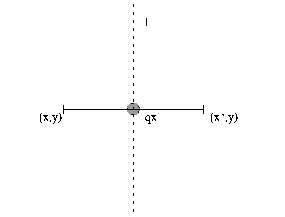
\includegraphics[scale=1.5]{images/interval_tree_query.pdf}
    \end{center}
    \caption{ — Consulta de um valor $q_x$ em um intervalo $[x, x']$}
    \label{fig:20}
\end{figure}


Segue o algoritmo (Algoritmo \ref{algo:8}) que recebe como parâmetros a raiz de uma árvore de intervalos $r$ e ponto para consulta $q_x$.

\begin{algorithm}[h!]
    \caption{Recebe a raiz de uma árvore de intervalos $r$ e um ponto de consulta $q_x$. Devolve todos os segmentos que contêm $q_x$.}
    \label{algo:8}
    \begin{algorithmic}[1]
        \Function{ConsultaÁrvoreDeIntervalos}{$r$, $q_x$}
            \If{$r$ não for folha}
                \If{$q_x$ for < $r$}
                    \State Consulte $\tau_{esq}(r)$ começando pelo intervalo com o ponto mais à esquerda e reporte todos intervalos que contenham $q_x$. Pare a consulta no primeiro intervalo que não contenha $q_x$.
                    \State \Call{ConsultaÁrvoreDeIntervalos}{$r_{esq}$, $q_x$}
                \Else
                    \State Consulte $\tau_{dir}(r)$ começando pelo intervalo com o ponto mais à direita e reporte todos intervalos que contenham $q_x$. Pare a consulta no primeiro intervalo que não contenha $q_x$.
                    \State \Call{ConsultaÁrvoreDeIntervalos}{$r_{dir}$, $q_x$}
                \EndIf
            \EndIf
        \EndFunction
    \end{algorithmic}
\end{algorithm}

Vamos acompanhar uma consulta na árvore construída da Figura \ref{fig:19}. Considere um ponto de consulta $q_x=1$. Iniciamos no nó$^0_1$. Como o nó não é folha, checamos se valor $q_x$ é menor que o $x_{med}$ salvo. O $x_{med}$ salvo é $14$, logo o ponto de consulta está à esquerda do nó$^0_1$. Consultamos $\tau_{esq}($nó$^0_1)$ e o intervalo $s_3$ não contém $q_x = 1$, portanto paramos a consulta em $\tau_{esq}($nó$^0_1)$. Então procedemos com a consulta no nó à esquerda. Note que ambos $q_x=1 \geq 1$ então consultaremos a lista $\tau_{dir}(r)$; reportando ambos $\{s_1,s_2\}$ que contêm 1.

\subsection{Árvore de Intervalos para consulta de segmentos no plano}

Seja $S$ o conjunto de $n$ segmentos no plano $P$ paralelos aos eixos de consulta. Para consultar quais segmentos de forma $s=(s_x,s_y)(s_x', s_y)$ estão dentro de uma janela de consulta $J = [x, x'] \times [y, y']$ podemos utilizar a estrutura de dados construída no capítulo \ref{cap:desenvolvimento}, as árvores de alcance, para encontrar quais dos $2n$ pontos extremos dos segmentos estão dentro da janela $J$. Contudo essa consulta não conseguiria encontrar segmentos que cruzam a janela, isto é, ambos pontos extremos estão fora da janela, porém passam por ela.

\begin{figure}[h!]
    \begin{center}
        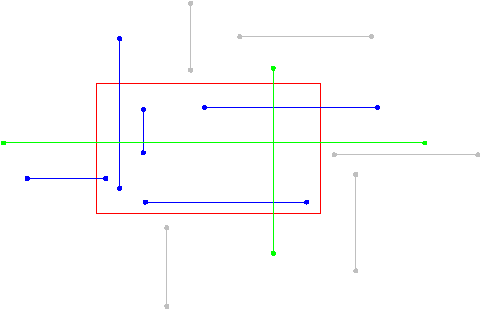
\includegraphics{images/interval_tree7.pdf}
    \end{center}
    \caption{ — Em azul: os segmentos encontrados pela árvore de alcance e que possuem pelo menos um ponto extremo dentro da janela. Em verde: os segmentos que cruzam as extremidades da janela e reportados pela árvore de intervalos. Em cinza, os segmentos que não devem ser reportados. Em vermelho : A janela de consulta}
    \label{fig:21}
\end{figure}

Para os segmentos que cruzam a janela, vistos em verde na Figura \ref{fig:21}, utilizaremos uma árvore de intervalos. Contudo, para uma consulta no plano, ela será modificada para que leve em consideração o comportamento bidimensional da consulta. Para isso adaptaremos as estruturas auxiliares $\tau_{esq}(r)$ e $\tau_{dir}(r)$.
Iremos montar o caso dos segmentos horizontais. Os verticais são simétricos; porém, na orientação vertical. Um segmento $s= (s_x,s_y) (s_x',s_y)$ que cruza as duas extremidades da janela $[x, x'] \times [y, y']$ tem seu ponto à esquerda de $x$, isto é, $s_x < x$ e similarmente seu ponto mais à direita é maior que $x'$, isto é,  $s_x' > x'$. Portanto, para saber se um segmento cruza a janela podemos escolher uma das extremidades da janela e fazer uma consulta para saber se o intervalo $[s_x, s_x']$ contém uma das extremidades da janela. Neste trabalho implementamos como \cite{cgi1} e consideramos a extremidade mais à esquerda da janela para consultas de segmentos horizontais. E a extremidade inferior da janela para consultas de segmentos verticais.
\begin{figure}[h]
\centering
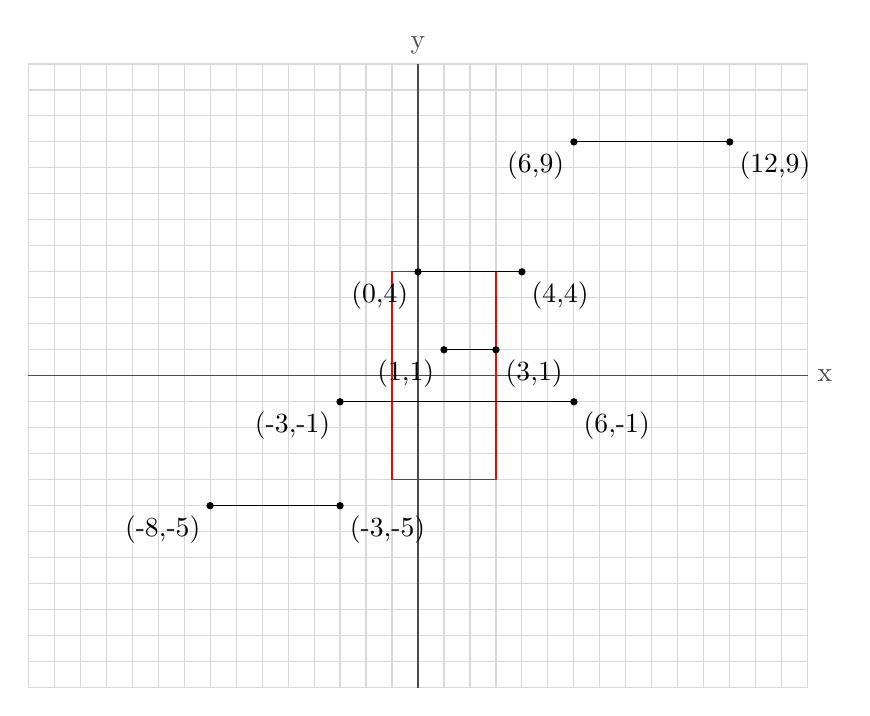
\begin{tikzpicture}[scale=0.33]
    \draw[gray!30] (-15,-12) grid[xstep=1, ystep=1]  (15,12);
    \draw[black!70] (-15,0)--(15,0) node[right]{x}; % x axis
    \draw[black!70] (0,-12)--(0,12) node[above]{y}; % y axis
    
    \draw[draw=red] (-1,4) rectangle (3,-4);

   \draw (0,4) -- (4,4);
   \draw (-8,-5) -- (-3,-5);
   \draw (6, 9) -- (12, 9);
   \draw (-3,-1) -- (6, -1);
   \draw (1,1) -- (3,1);4
   
   \fill (0,4)  circle[radius=4pt] node[anchor=north east]{(0,4)};
   \fill (4,4)  circle[radius=4pt] node[anchor=north west]{(4,4)};
   \fill (-8,-5)  circle[radius=4pt] node[anchor=north east]{(-8,-5)};
   \fill (-3,-5)  circle[radius=4pt] node[anchor=north west]{(-3,-5)};
   \fill (6,9)  circle[radius=4pt] node[anchor=north east]{(6,9)};
   \fill (12,9)  circle[radius=4pt] node[anchor=north west]{(12,9)};
   \fill (-3,-1)  circle[radius=4pt] node[anchor=north east]{(-3,-1)};
   \fill (6,-1)  circle[radius=4pt] node[anchor=north west]{(6,-1)};
   \fill (1,1)  circle[radius=4pt] node[anchor=north east]{(1,1)};
   \fill (3,1)  circle[radius=4pt] node[anchor=north west]{(3,1)};
   
\end{tikzpicture}
\caption {Em vermelho a região do retângulo de consulta}
\label{fig:23}
\end{figure}

A construção de uma árvore de intervalos para consulta de segmentos no plano é a mesma para intervalos na reta real. A diferença é a estrutura auxiliar. Ao invés de uma lista ordenada, usaremos uma árvore de alcance. Construímos uma árvore de alcance com os pontos mais à esquerda dos segmentos de $I_{med}$ e guardamos em $\tau_{esq}$; De forma análoga construímos uma árvore de alcance com os pontos mais à direita dos segmentos de $I_{med}$.

Vamos considerar o conjunto de segmentos no plano da Figura \ref{fig:23} para ilustrar a construção da árvore de intervalos para segmentos no plano.
Inicialmente vamos ordenar os intervalos de $I$ pelo ponto mais à esquerda: $s_1 = [(-8,-5)(-3,-5)]$, $s_2 =[(-3,-1)(6, -1)]$, $s_3 = [(0,4)(4,4)]$, $s_4 =[(1,1)(3,1)]$, $s_5 = [(6,9)(12,9)]$. Criamos um nó raiz $r$ e nele armazenamos o valor da $x_{med}  = 1$. Dividimos o conjunto de intervalos em três subconjuntos: $I_{esq}$ com o segmento $\{s_1\}$, $I_{dir}$ com o segmento $\{s_5\}$ por fim $I_{med}$ com os segmentos, que contem $x_{med}$, $\{ s_2, s_3, s_4\}$. Isto é, a $x$-coordenada do segmento está entre o valor $x_{med}$.Construímos uma árvore de alcance com os segmentos de $I_{med}$ em relação aos pontos mais à esquerda dos segmentos e associamos esta árvore a $\tau_{esq}(r)$. Construímos outra árvore de alcance com os segmentos de $I_{med}$ considerando os pontos mais à direita e associamos a $\tau_{dir}(r)$. A subárvore à esquerda será uma árvore de intervalos sobre $I_{esq}$; e a subárvore à direita será uma árvore de intervalos sobre $I_{dir}$. A seguir a Figura \ref{fig:24} ilustra a árvore de intervalos construída. Na Figura \ref{fig:range_tree_right_assoc_interval} temos um exemplo da árvore mais externa da árvore de alcance construída sob os pontos extremos mais à direita dos intervalos no nó$^0_1$.
 
\begin{figure}[h!]
    \begin{center}
        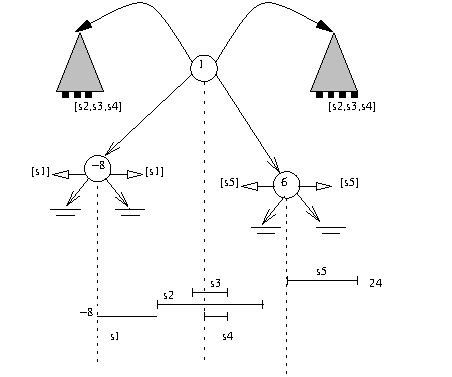
\includegraphics[scale=1.5]{images/interval_tree9.pdf}
    \end{center}
    \caption{ Árvore de intervalos construída com os segmentos da Figura \ref{fig:23}}
    \label{fig:24}
\end{figure}

\begin{figure}[h!]
    \centering
    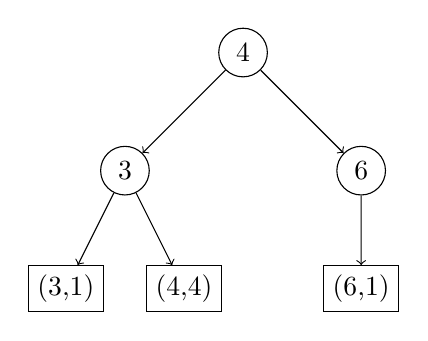
\begin{tikzpicture}[nodes={draw, circle}, ->]
    % Tree structure
 \node{4}
        child { node {3} 
                child{ node[rectangle]{(3,1)}}
                child{ node[rectangle]{(4,4)}}
        }
        child [missing]
        child { node {6}
            child{ node[rectangle]{(6,1)}}
        };
\end{tikzpicture}
    \caption{A árvore de alcance mais externa construída com os pontos extremos à direita associada à direita do nó$^0_1$ da árvore de intervalos da Figura \ref{fig:24}.}
    \label{fig:range_tree_right_assoc_interval}
\end{figure}



\subsection{Consulta para encontrar segmentos em janela}
Para obter os segmentos do conjunto $S$ com $n$ segmentos no plano e que estão contidos em uma a janela $J=[x,x']\times[y, y']$ iremos primeiro consultar uma árvore de alcance construída sobre os $2n$ pontos extremos (todos os pontos de todos os segmentos). Neste trabalho modificamos a árvore de alcance para que construa na raiz um mapa $ponto \rightarrow segmento$. Durante a consulta da árvore de alcance, está retornará todos os pontos dentro da janela e acessamos esse mapa da raiz para saber quais são os segmentos associados aos pontos encontrados. Obtemos assim os segmentos que tem ao menos um ponto dentro da janela.

Para obtermos os segmentos cujos pontos extremos estão fora da janela de consulta utilizaremos a árvore de intervalos construída anteriormente. Consultamos a estrutura auxiliar com uma janela que garante que o ponto do segmento cruza uma das laterais da janela. A consulta em $\tau_{esq}(r)$ será com a janela $J'_{-\infty}=]-\infty, x] \times [y, y']$. Similarmente a consulta na árvore associada $\tau_{dir}(r)$  $J'_{\infty}=[x', \infty[ \times [y, y']$. A Figura \ref{fig:fig22} ilustra a janela $J'_{-\infty}$ de consulta. Logo depois descrevemos um algoritmo que consulta a árvore de intervalos e as estruturas associadas.

\begin{figure}[h!]
    \centering

    \tikzset{every picture/.style={line width=0.75pt}} %set default line width to 0.75pt        
    
    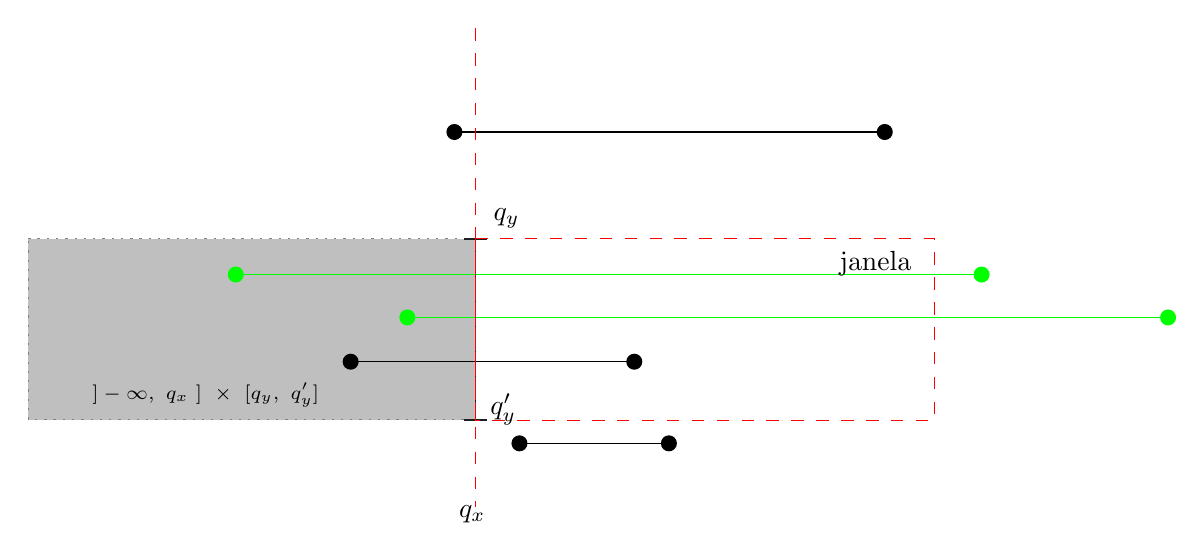
\begin{tikzpicture}[x=0.75pt,y=0.75pt,yscale=-1,xscale=1]
    %uncomment if require: \path (0,268); %set diagram left start at 0, and has height of 268
    
    %Shape: Rectangle [id:dp6848378981286898] 
    \draw  [color={gray}  ,draw opacity=1 ][fill={gray}  ,fill opacity=0.5 ][dash pattern={on 0.84pt off 2.51pt}] (56.33,111.67) -- (271.67,111.67) -- (271.67,199) -- (56.33,199) -- cycle ;
    %Straight Lines [id:da6014347269241187] 
    \draw [color={green}  ,draw opacity=1 ]   (605.5,149.67) -- (239,149.67) ;
    \draw [shift={(239,149.67)}, rotate = 180] [color={green}  ,draw opacity=1 ][fill={green}  ,fill opacity=1 ][line width=0.75]      (0, 0) circle [x radius= 3.35, y radius= 3.35]   ;
    \draw [shift={(605.5,149.67)}, rotate = 180] [color={green}  ,draw opacity=1 ][fill={green}  ,fill opacity=1 ][line width=0.75]      (0, 0) circle [x radius= 3.35, y radius= 3.35]   ;
    %Straight Lines [id:da9755427473669658] 
    \draw    (348.33,171) -- (211.67,171) ;
    \draw [shift={(211.67,171)}, rotate = 180] [color={rgb, 255:red, 0; green, 0; blue, 0 }  ][fill={rgb, 255:red, 0; green, 0; blue, 0 }  ][line width=0.75]      (0, 0) circle [x radius= 3.35, y radius= 3.35]   ;
    \draw [shift={(348.33,171)}, rotate = 180] [color={rgb, 255:red, 0; green, 0; blue, 0 }  ][fill={rgb, 255:red, 0; green, 0; blue, 0 }  ][line width=0.75]      (0, 0) circle [x radius= 3.35, y radius= 3.35]   ;
    %Straight Lines [id:da9291827808721727] 
    \draw    (365,210.33) -- (293,210.33) ;
    \draw [shift={(293,210.33)}, rotate = 180] [color={rgb, 255:red, 0; green, 0; blue, 0 }  ][fill={rgb, 255:red, 0; green, 0; blue, 0 }  ][line width=0.75]      (0, 0) circle [x radius= 3.35, y radius= 3.35]   ;
    \draw [shift={(365,210.33)}, rotate = 180] [color={rgb, 255:red, 0; green, 0; blue, 0 }  ][fill={rgb, 255:red, 0; green, 0; blue, 0 }  ][line width=0.75]      (0, 0) circle [x radius= 3.35, y radius= 3.35]   ;
    %Straight Lines [id:da8381433224809642] 
    \draw    (469,60.33) -- (261.67,60.33) ;
    \draw [shift={(261.67,60.33)}, rotate = 180] [color={rgb, 255:red, 0; green, 0; blue, 0 }  ][fill={rgb, 255:red, 0; green, 0; blue, 0 }  ][line width=0.75]      (0, 0) circle [x radius= 3.35, y radius= 3.35]   ;
    \draw [shift={(469,60.33)}, rotate = 180] [color={rgb, 255:red, 0; green, 0; blue, 0 }  ][fill={rgb, 255:red, 0; green, 0; blue, 0 }  ][line width=0.75]      (0, 0) circle [x radius= 3.35, y radius= 3.35]   ;
    %Straight Lines [id:da7444817332368282] 
    \draw [color={green}  ,draw opacity=1 ]   (515.67,129) -- (156.33,129) ;
    \draw [shift={(156.33,129)}, rotate = 180] [color={green}  ,draw opacity=1 ][fill={green}  ,fill opacity=1 ][line width=0.75]      (0, 0) circle [x radius= 3.35, y radius= 3.35]   ;
    \draw [shift={(515.67,129)}, rotate = 180] [color={green}  ,draw opacity=1 ][fill={green}  ,fill opacity=1 ][line width=0.75]      (0, 0) circle [x radius= 3.35, y radius= 3.35]   ;
    %Straight Lines [id:da4271924427932462] 
    \draw [color={rgb, 255:red, 30; green, 30; blue, 30 }  ,draw opacity=1 ]   (271.67,111.67) -- (271.67,199) ;
    \draw [shift={(271.67,199)}, rotate = 270] [color={rgb, 255:red, 30; green, 30; blue, 30 }  ,draw opacity=1 ][line width=0.75]    (0,5.59) -- (0,-5.59)   ;
    \draw [shift={(271.67,111.67)}, rotate = 270] [color={rgb, 255:red, 30; green, 30; blue, 30 }  ,draw opacity=1 ][line width=0.75]    (0,5.59) -- (0,-5.59)   ;
    %Straight Lines [id:da33530800628578705] 
    \draw [color={red },draw opacity=1 ] [dash pattern={on 4.5pt off 4.5pt}]  (271.67,10.33) -- (271.67,113.5) -- (271.67,241) ;
    %Shape: Rectangle [id:dp2955317576076706] 
    \draw  [color={red},draw opacity=1 ][dash pattern={on 4.5pt off 4.5pt}] (271.67,111.67) -- (493,111.67) -- (493,199.33) -- (271.67,199.33) -- cycle ;
    % Text Node
    \draw (262.67,239.07) node [anchor=north west][inner sep=0.75pt]    {$q_{x}$};
    % Text Node
    \draw (86,180.07) node [anchor=north west][inner sep=0.75pt]  [font=\scriptsize]  {$] -\infty ,\ q_{x} \ ] \ \times \ [ q_{y} ,\ q_{y} ']$};
    % Text Node
    \draw (279.33,96.07) node [anchor=north west][inner sep=0.75pt]    {$q_{y}$};
    % Text Node
    \draw (277.67,185.07) node [anchor=north west][inner sep=0.75pt]    {$q_{y} '$};
    % Text Node
    \draw (446,116.67) node [anchor=north west][inner sep=0.75pt]   [align=left] {janela};
    \end{tikzpicture}
    \caption{Consulta na árvore de intervalos para segmentos que cruzam a janela. Em verde os segmentos que queremos reportar com esta consulta}
    \label{fig:fig22}
\end{figure}

\begin{algorithm}[h!]
    \caption{Recebe a raiz de uma árvore de intervalos $r$ e uma janela de consulta $J=[x,x']\times[y, y']$. Devolve todos os segmentos que atravessam $J$.}
    \begin{algorithmic}[1]
        \Function{ConsultaÁrvoreDeIntervalosNoPlano}{$r$, $J$}
            \If{$r$ não for folha}
                %\If{$q_x$ for < $r$}
                \If{$x$  < $r$}
                    %\State Consulte
                    \State $L_e\leftarrow$\Call{BuscaEmAlcance2D}{$\tau_{esq}(r)$ , $]-\infty, x] \times [y, y']$}
                    \State Verifique se o ponto direito de cada elemento de $L_e$ é maior que $x'$.
                    \State \Call{ConsultaÁrvoreDeIntervalosNoPlano}{$r_{esq}$, $J$}
                \Else
                    \State $L_d\leftarrow$ \Call{BuscaEmAlcance2D}{$\tau_{dir}(r)$ , $[x', \infty [ \times [y, y']$}
                    \State Verifique se o ponto esquerdo de cada elemento de $L_d$ é menor que $x$.
                    \State \Call{ConsultaÁrvoreDeIntervalosNoPlano}{$r_{dir}$, $J$}
                \EndIf
            \EndIf
        \EndFunction
    \end{algorithmic}
\end{algorithm}

Vamos acompanhar uma consulta na árvore construída para a Figura \ref{fig:23}. Inicialmente queremos descobrir quais segmentos tem ao menos um ponto extremo dentro da janela. Consultamos a árvore de alcance construída com os $2n$ pontos com a janela $J=[-1,3]\times[-4,4]$. Esta consulta devolve $(1,1), (3,1), (0,4)$; consultamos o mapa na raiz da árvore e devolvemos os segmentos $[s_3, s_4]$. Seguimos para a consulta da árvore de intervalos. Iniciamos na raiz nó$^0_1$. Como o nó não é folha, checamos se $-1$ (a extremidade esquerda da janela) é menor que o $x_{med}$ salvo no nó. O $x_{med}$ salvo é 1, logo a consulta está à esquerda de nó$^0_1$. Consultamos a árvore associada $\tau_{esq}($nó$^0_1)$ com a janela  $]-\infty, -1] \times [-4, 4]$ devolvendo $(-3, -1)$; utilizando o mapa associado à raiz devolvemos o segmento $[s_2]$.
A Figura \ref{fig:fig25} mostra os resultados obtidos com a nossa implementação para consultar segmentos horizontais no plano.

\begin{figure}[h]
\centering
\begin{minipage}{.5\textwidth}
  \centering
  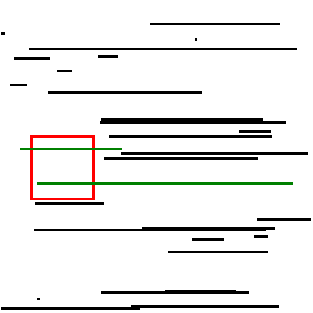
\includegraphics[width=.8\linewidth]{images/inside_segments.pdf}

  \label{fig:test1}
\end{minipage}%
\begin{minipage}{.5\textwidth}
  \centering
  
  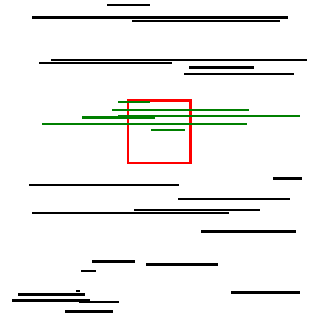
\includegraphics[width=.8\linewidth]{images/inside_segments2.pdf}
  \label{fig:test2}
 
\end{minipage}
 \caption{Resultados das consultas em janela com Árvore de Intervalos no plano}
 \label{fig:fig25}
\end{figure}

%\clearpage

\section{Árvore de Segmentos}
Em uma consulta em janela, na seção \ref{interval-tree}, a Árvore de Intervalos nos foi útil para encontrar segmentos paralelos aos eixos da consulta. A primeira vista podemos pensar que conseguimos encontrar segmentos com quaisquer orientações com esta estrutura considerando cada segmento apenas suas componentes cartesianas $x$-intervalo e $y$-intervalo. No melhor caso, esta alternativa funcionará bem e a maioria dos segmentos terá suas componentes intersectando a janela. No pior dos casos, a consulta reportaria segmentos que possui componentes que tanto seu $x$-intervalo quanto seu $y$-intervalo respeitam a consulta em janela, porém, o segmento não necessariamente cruza a consulta. Como por exemplo na figura \ref{fig:interval_tree_worst_case}.

\begin{figure}[h!]
    \centering
    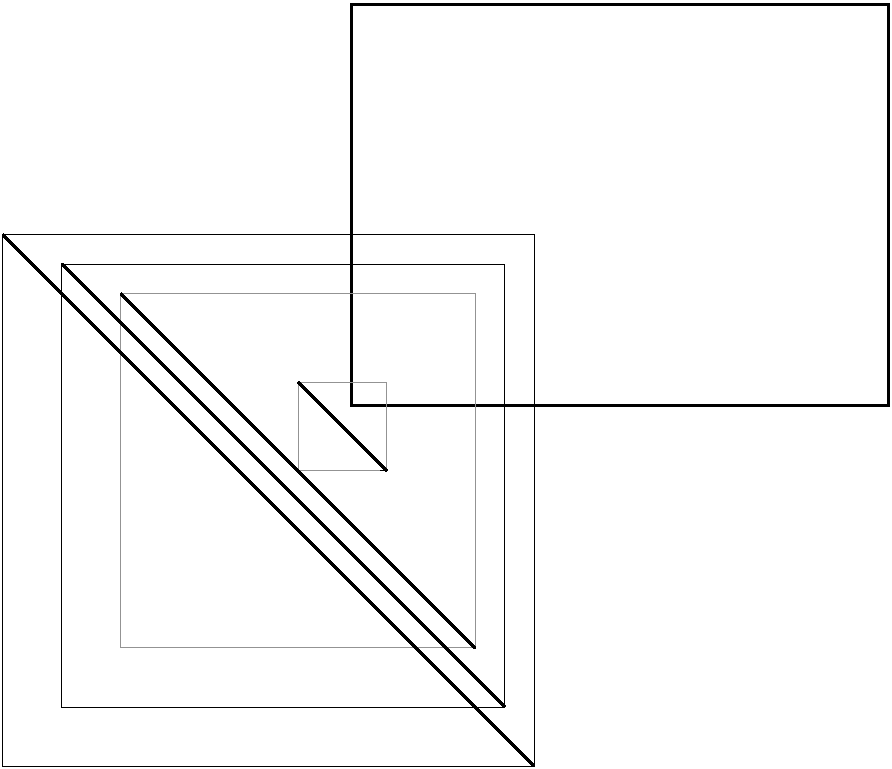
\includegraphics[scale=0.5]{images/interval_tree_fail.pdf}
    \caption{Consulta de segmentos com inclinação e com árvore de intervalos no pior caso. Em vermelho a janela de consulta.}
    \label{fig:interval_tree_worst_case}
\end{figure}

Para conseguirmos consultar segmentos com inclinação adotaremos a mesma estratégia da seção \ref{interval-tree}. Iremos portanto distinguir segmentos que tem um ponto extremo dentro da janela de segmentos que cruzam as extremidades da janela. O primeiro caso conseguimos reportar com uma árvore de alcance. Para encontrar o segundo tipo de segmento iremos realizar uma consulta de intersecção com cada uma das quatro arestas que compõem a janela. Iremos demonstrar como realizar consultas apenas com uma borda vertical. Para consultas sobre as bordas horizontais, uma abordagem simétrica pode ser utilizada. Uma árvore de segmentos pode ser construída em tempo de ordem $O(n\log(n))$. A consulta consegue reportar todos os segmentos que intersectam a janela em tempo $O(\log^2(n) +k)$ onde $k$ é o numero de segmentos reportados \cite{cg08}.

\subsection{Árvores de Segmentos para consultas unidimensionais}
%A construção de uma árvore de segmentos é uma adaptação para árvore de intervalos. Consultando em uma árvore de intervalos $v$ por $q = q_x \times [q_y, q_y']$ obtemos $I_{mid}(v)$. Sabemos que um segmento cruza uma consulta $q_x$ apenas consultando $I_{mid}(v)$, e consultando o intervalo $[q_y, q_y']$. Esta alternativa falha para pontos com orientação pois não conseguimos garantir que mesmo se o outro ponto extremo do segmento estiver dentro da do intervalo $[q_y, q_y']$ o segmento cruzará a janela.

Vamos %então 
reduzir o problema de consulta em uma janela $J = [q_x, q_x'] \times [q_y, q_y']$ para quatro consultas unidimensionais. Vamos construir uma árvore de segmentos para reta real, e depois expandimos para o plano. Seja $I={[x_1, x_1'], [x_2, x_2'], ... , [x_n, x_n'] }$ o conjunto dos $n$ intervalos na reta real. Queremos construir uma estrutura de dados capaz de retornar os intervalos que contêm $q_x$. Seja $p_1, p_2, ..., p_m$ a lista de todos os pontos extremos de cada intervalo, ordenados do menor para o maior. Iremos construir a partir dos $m$ pontos dos intervalos de $I$ um conjunto de intervalos elementares. Os intervalos elementares consistem de intervalos abertos entre dois pontos extremos consecutivos $p_i$ e $p_{i+1}$, alternados com um intervalo unitário fechado de apenas um ponto extremo $[p_i, p_i]$. A razão para tratarmos os pontos extremos como intervalos fechados é pelo fato de a resposta da consulta não ser necessariamente a mesma dentro de um intervalo e nos seus pontos extremos. Iremos então construir uma árvore binaria $\tau$ em que suas folhas armazenam os intervalos elementares. Denotaremos o intervalo correspondente de uma folha $\mu$ como $Int(\mu)$.
\[
    ]-\infty, p_1[, [p_1, p_1], ]p_1, p_2[, [p_2, p_2] ... , ]p_{m-1}, p_m[, [p_m, p_m], ]p_m, +\infty [
\]

\begin{figure}[h!]
    \centering
    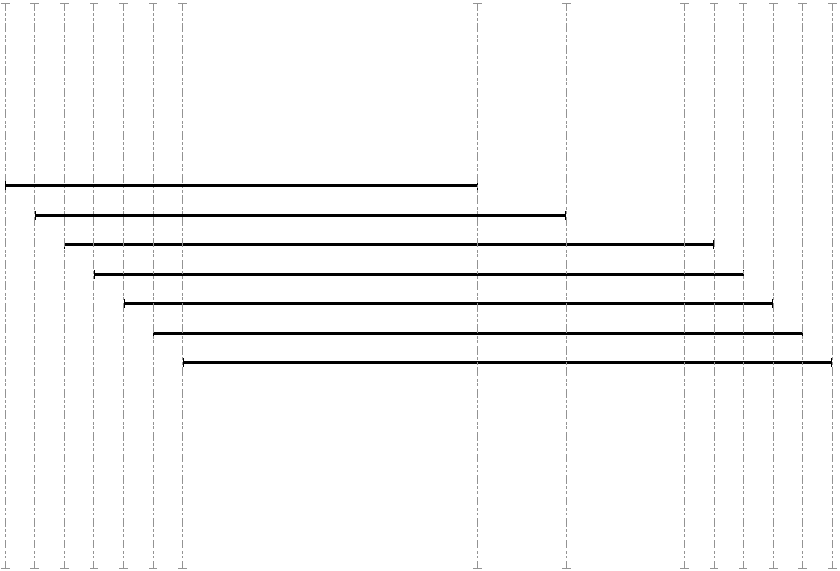
\includegraphics[scale=0.4]{images/elementary_segments.pdf}
    \caption{Intervalos no plano seccionados em cada $p_n$ }
    \label{fig:intervals_sected}
\end{figure}

Há também um intervalo associado a cada nó não folha que é formado pela a união dos intervalos dos nós filhos. Logo, o intervalo associado à raiz da árvore de segmentos é o intervalo $]-\infty, +\infty[$. Chamaremos o nó $v$ que guarda o valor $[p, p_i']$ de $v_{p, p_i'}$.  Munidos da árvore binária balanceada $\tau$ construída com os intervalos elementares, inserimos cada intervalo $i$ na árvore $\tau$ de forma que o nó $v_{p_i, p_i'} \subseteq i$. Como um intervalo pode conter muitos intervalos elementares. A figura \ref{fig:segment_tree1} mostra a quantidade de intervalos elementares contidos em um segmento $s$. Note que é bom armazenar $s$ no nó $v$ pois $s$ contém todos os intervalos elementares obtidos a partir de $v$. %como um intervalo fica representado na árvore de segmentos.

\begin{figure}[h!]
    \centering
    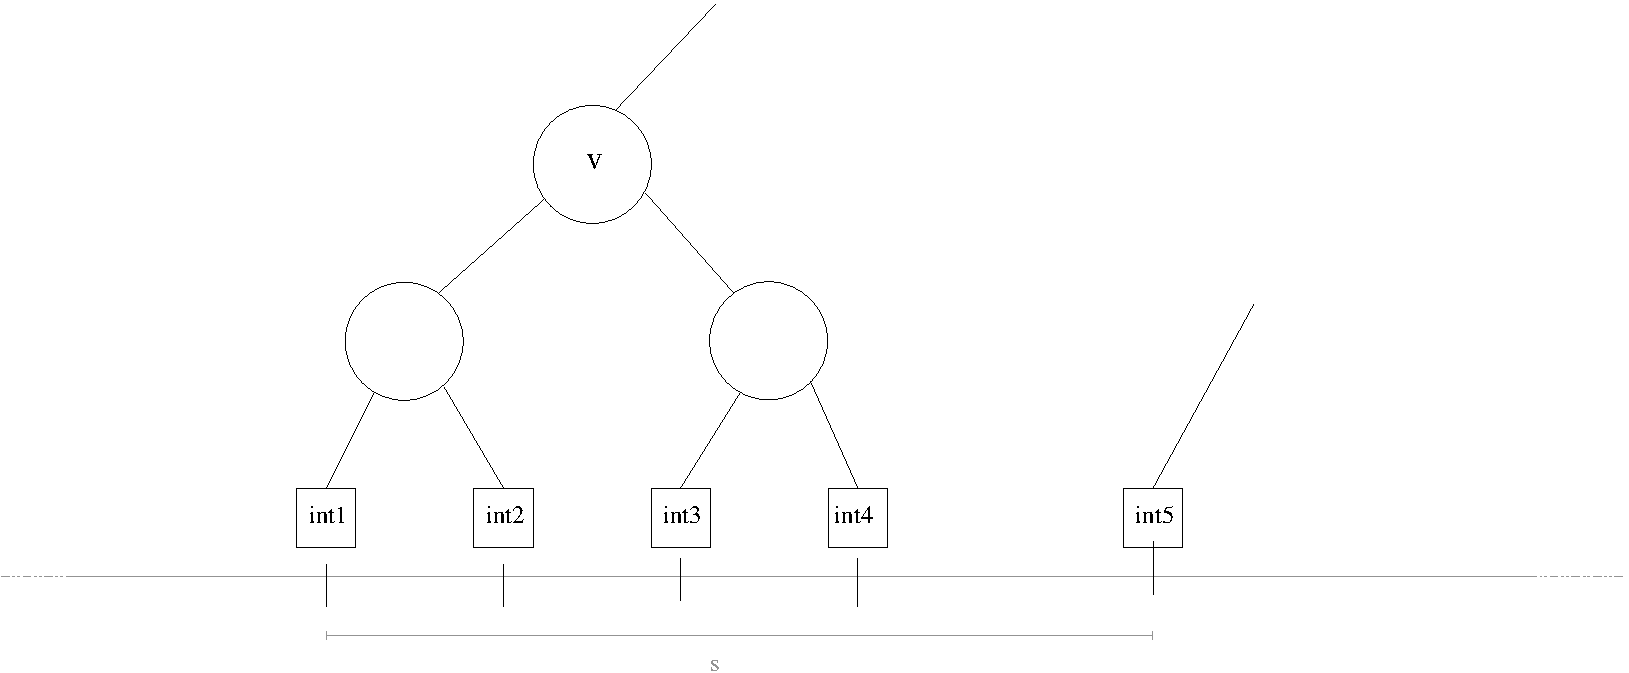
\includegraphics[scale=0.5]{images/elementary_seg_tree.pdf}
    \caption{Árvore de segmentos representando um intervalo $s$ }
    \label{fig:segment_tree1}
\end{figure}

A construção de uma árvore binária balanceada será feita de baixo-para-cima. Construímos uma fila $f$ com os intervalos elementares ordenados pelo seu valor mais à esquerda. Ao iniciar a construção pegaremos os dois primeiros valores de $f$, unimos seus intervalos e colocamos novamente no fim da fila. Fazemos isto até restar somente um intervalo. Segue um procedimento na Figura \ref{fig:building-bottom-up} para a construção da árvore de segmentos para intervalos unidimensionais.
Porém, o numero de intervalos elementares nesta fila deve ser potencia de 2 pois somente assim conseguiremos construir a árvore par-a-par. Ou seja, para conseguirmos construir a árvore baixo-cima precisamos antes unir intervalos elementares até que o numero de intervalos seja uma potencia de 2. Fazemos isso percorrendo a fila e unindo intervalos par-a-par ordenadamente e preservando sua posição na fila.

\begin{figure}[h!]
    \centering
    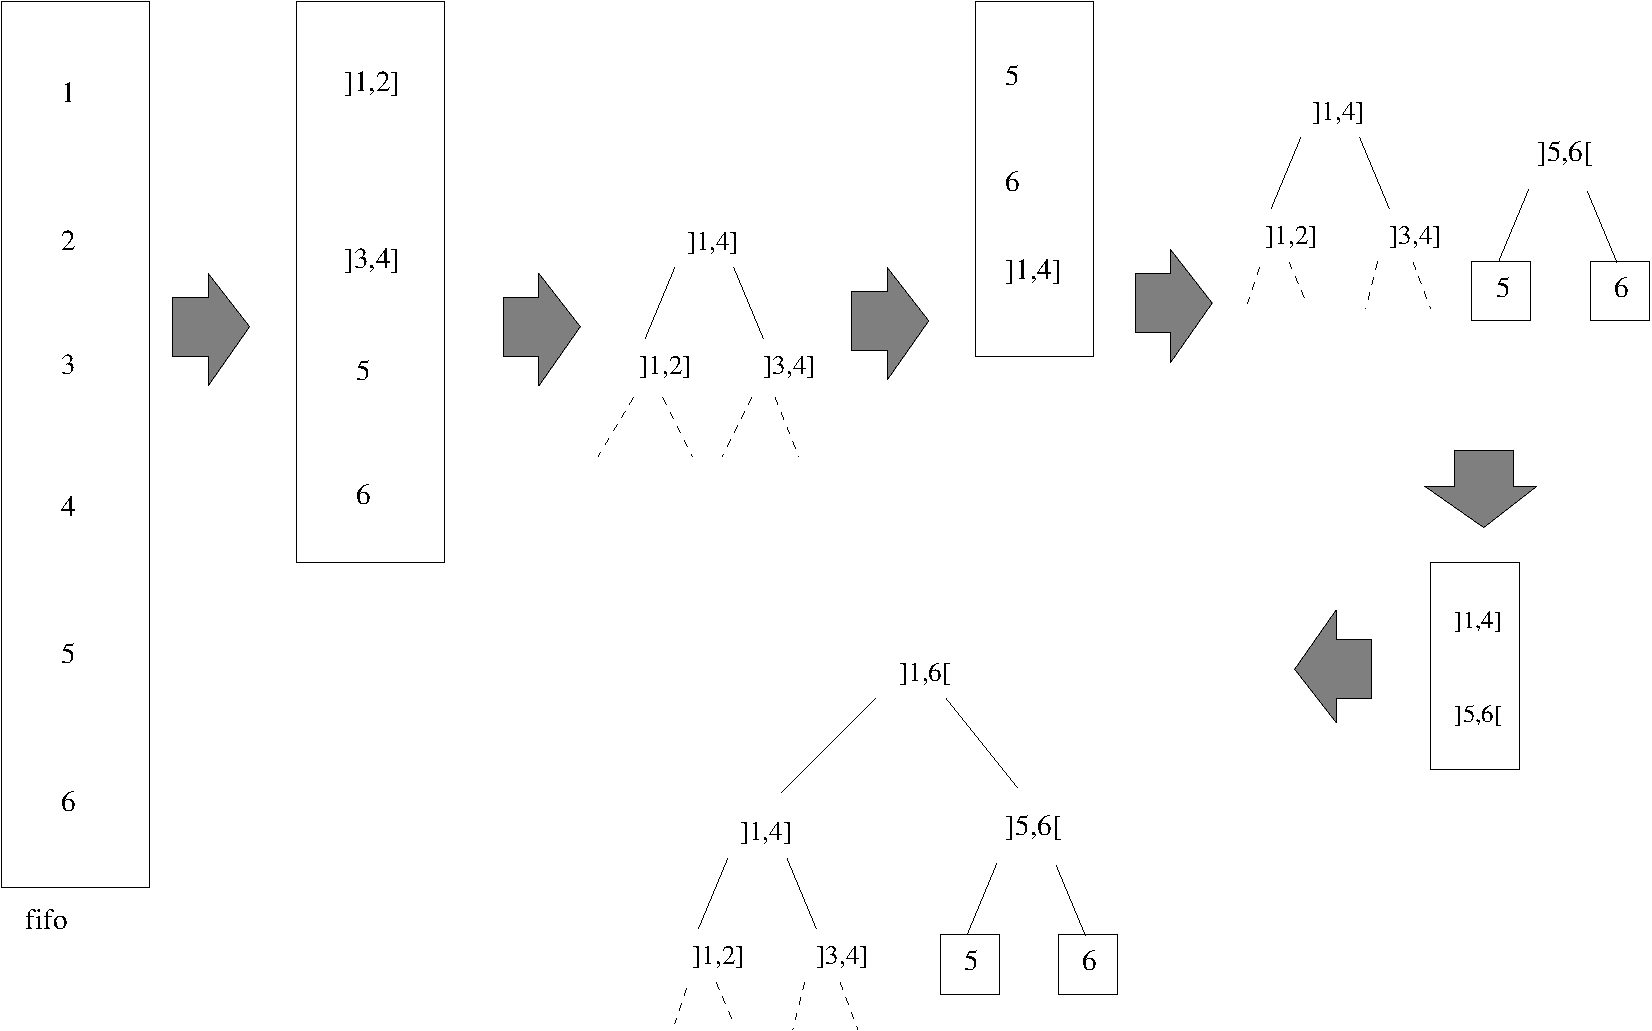
\includegraphics[scale=0.55]{images/fifo_update.pdf}
    \caption{Construímos a árvore de baixo-para-cima juntando elementos da fila par-a-par}
    \label{fig:building-bottom-up}
\end{figure}

\begin{algorithm}[h!]
    \caption{Recebe uma lista de intervalos elementares $I$ ordenada, retorna a fila de nós de tamanho $\lfloor(\log_2n)\rfloor$ com intervalos unidos}
    \begin{algorithmic}[1]
        \Function{ConstróiFilaAuxiliar}{$I$}
            \State Coloque todos os intervalos elementares (em ordem) em uma fila 
            \State Calcule tamanho mínimo da fila: $t_{min} = 2^{\lfloor(\log_2{|I|})\rfloor)}$
            \State Inicie um contador
            \While{ $|I| > t_{min}$}
                \State Remova da fila os intervalos elementares $n$ e $n+1$
                \State Crie um nó $v$, e guarde o seu valor com a união do intervalo elementar $n$ e de $n+1$
                \State Associe à subárvore a esquerda de $v$ um nó folha com o valor do intervalo $n$
                \State Associe à subárvore a direita de $v$ um nó folha com o valor do intervalo $n+1$
                \State Insira o nó $v$ na posição $n$.
                \State Incremente o contador
            \EndWhile
        \EndFunction
    \end{algorithmic}
\end{algorithm}
 Por fim, teremos uma árvore binária $\tau$ com intervalos elementares como folhas. Precisamos inserir os intervalos nos nós. Para cada nó $v$ da árvore iremos inserir o intervalo $[x, x']$ se o $Int(v) \subseteq [x, x']$ e o $pai(v) \nsubseteq [x, x']$. A árvore seguindo estes princípios é chamada de árvore de segmentos.  A seguir o algoritmo para inserir os intervalos na árvore $\tau$.
 
 
\begin{algorithm}[h!]
    \caption{Recebe a raiz de uma árvore binária de intervalos elementares $v$, e um intervalo $s = [x, x']$. Retorna a raiz $v'$ com o intervalo inserido nos nós cujo $Int(v) \subseteq  s$}
    \begin{algorithmic}[1]
        \Function{InsereSegmentoÁrvoreSegmentos}{$v$, $[x, x']$}
            \If{$Int(v) \subseteq [x, x']$}
                \State Guarde o valor de $s$ em $v$
            \Else
                \If{$filho_{esq}(v) \cap [x, x'] \neq \emptyset $}
                    \State \Call{InsereSegmentoÁrvoreSegmentos}{$filho_{esq}(v), s$}
                \EndIf
                
                \If{$filho_{dir}(v) \cap [x, x'] \neq \emptyset $}
                    \State \Call{InsereSegmentoÁrvoreSegmentos}{$filho_{dir}(v), s$}
                \EndIf
            \EndIf
        \EndFunction
    \end{algorithmic}
\end{algorithm}

\begin{figure}
    \centering
    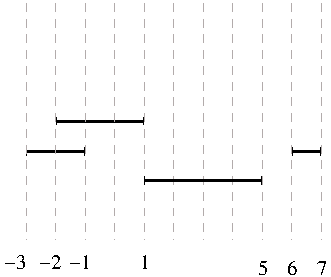
\includegraphics[scale=0.8]{images/exemple_segments.pdf}
    \caption{Intervalos na reta real}
    \label{fig:intervals}
\end{figure}

Seja $I$ o conjunto de intervalos da Figura \ref{fig:intervals}. Iniciamos construindo o conjunto de intervalos elementares: $]-\infty, -3[$ , $[-3, -3]$, $]-3, -2[$, $[-2,-2]$, $]-2, -1[$, $[-1, -1],\dots, ]6, 7[$, $[7,7]$, $]7, \infty [$. Inserimos na fila $f$ ordenadamente. Neste caso, o tamanho da fila é $15$, e para construirmos a árvore, precisamos reduzir para $2^{\lfloor(\log_2{15})\rfloor} = 2^3 = 8$ elementos na fila. Para isto, vamos iterar sobre nossa fila e unir os intervalos elementares $]-\infty, -3[$ e $[-3, -3]$. Criamos um nó $v$ e valor da união dos intervalos elementares é guardado no nó. $Int(v) = ]-\infty, -3]$. Atribuímos a subárvore à esquerda com o menor intervalo elementar e à direita o maior. E iteramos o próximo valor da fila.
Com a fila com tamanho $8$, conseguimos construir a árvore com a estratégia de baixo-para-cima. Iniciamos pegando da fila os dois primeiros elementos, unimos e adicionamos no fim da fila. Repetimos até restar apenas um elemento. Por fim, teremos a árvore da Figura \ref{fig:segment_tree2} a seguir.
Agora iremos inserir na árvore os intervalos do conjunto $I$. Para inserir $[-3, -1]$, começamos pela raiz $v_{-\infty, +\infty}$. Checamos se $ ]-\infty, +\infty[ \subseteq [-3, -1] $, como não é verdade, checamos se o $filho_{esq}(v) \cap [-3,-1] \neq \emptyset$ e se $filho_{esq}(v) \cap [-3,-1]\neq \emptyset$. Sendo verdade apenas para a primeira verificação. Chamamos recursivamente \Call{InsereSegmentoNaÁrvore}{$filho_{esq}(v_{-\infty, +\infty})$, $[-3, -1]$} e seguimos com a inserção. O intervalo $[-3,-1]$ não contém o  nó $]-\infty, 1]$, e ambos $filho_{esq}(v) = ]-\infty, -2] $ e $filho_{dir}(v) = ]-2, 1]$ intersectam o intervalo $s = [-3, -1]$. Chamamos recursivamente \Call{InsereSegmentoNaÁrvore}{$filho_{esq}(v_{- \infty, 1}, [-3, -1])$} e \Call{InsereSegmentoNaÁrvore}{$filho_{dir}(v_{- \infty, 1}, [-3, -1])$}. Segue-se estas consultas recursivas até chegar aos nós folhas. Os nós $v_{-3 -3}, v_{-3, -2}, v_{-2, -1}, v_{-1, -1}$ contêm o intervalo e portanto o intervalo é associado a estes nós.
A figura a seguir é uma ilustração da  árvore de segmento construída.
\begin{figure}[h!]
     \centering
     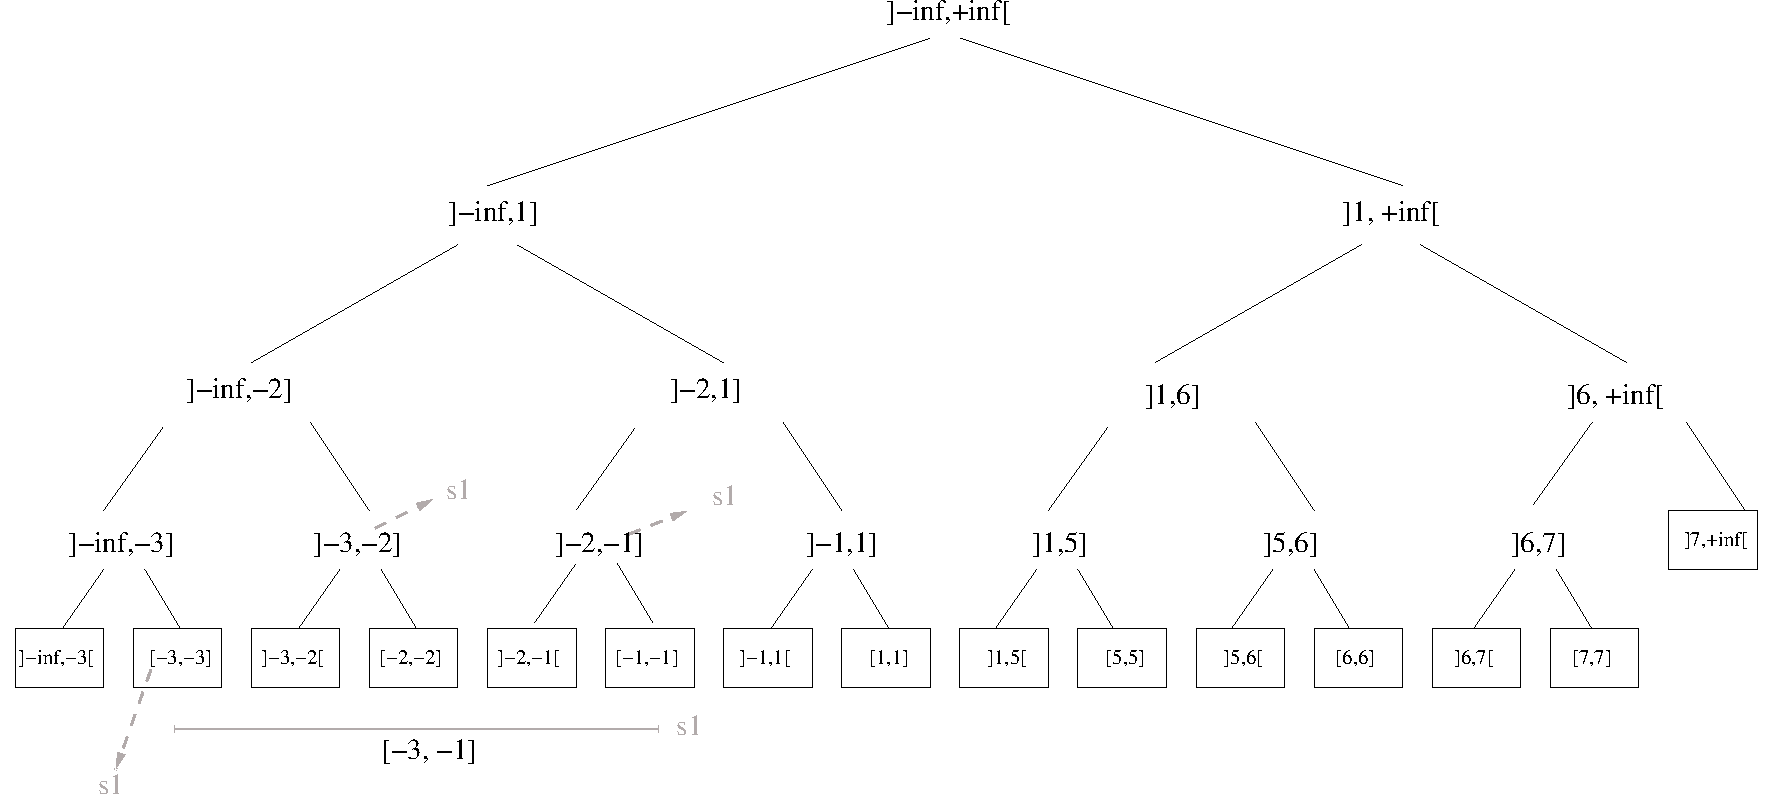
\includegraphics[scale=0.5]{images/arvore_seg.pdf}
     \caption{Árvore de segmentos construída}
     \label{fig:segment_tree2}
 \end{figure}

\subsection{Consulta unidimensional na Árvore de Segmentos}
Para consultar na Árvore construída queremos reportar todos os intervalos $s= [x, x']$ que intersectam a consulta $q = q_x$. Iremos consultar cada nó da árvore e enquanto não for nó folha, checaremos se o $Int(v)$ intersecta a consulta. Em cada visita a um nó, reportamos (se houver algum) os intervalos guardados no nó. A seguir o algoritmo para consulta em uma árvore de segmentos.

\begin{algorithm}[h!]
    \caption{Recebe a raiz de uma árvore de segmentos $v$, e um valor de consulta $q_x$. Retorna todos os intervalos que contem o ponto $q_x$}
    \begin{algorithmic}[1]
        \Function{ConsultaArvoreSegmentos}{$v$, $q_x$}
            \State Reporte os segmentos guardados em $v$.
            \If{$v$ não é folha}
                \If{$q_x$ \in $Int(filho_{esq}(v))$}
                    \State \Call{ConsultaArvoreSegmentos}{$filho_{esq}(v)$, $q_x$}
                \Else
                    \State \Call{ConsultaArvoreSegmentos}{$filho_{dir}(v)$, $q_x$}
                \EndIf
            \EndIf
        \EndFunction
    \end{algorithmic}
\end{algorithm}

Vamos acompanhar uma consulta na árvore construída para a Figura \ref{fig:segment_tree2} para o ponto $q_x=-1$. Iniciamos na raiz $v_{-\infty, + \infty}$, e não há segmentos para serem reportados. Consultamos se o intervalo da subárvore à esquerda intersecta $-1$. Consultamos recursivamente agora a subárvore à esquerda. Não há intervalos para serem reportados. Consultamos se $-1 \in filho_{esq}(v_{-\infty, -2})$, o que é falso então consultamos $filho_{dir}(v) $. Seguimos recursivamente para $v_{-\infty, -3}$ reportamos os segmentos e seguimos com a consulta recursiva. Consultamos recursivamente se $-1 \in filho_{esq}(v) = ]-\infty, -3]$, o que é falso. E consultamos o nó $filho_{dir}(v) = [-3, -3]$ e retornamos o segmento associado $S_1$.

\subsection{Estendendo a Árvore de segmentos para janelas 2D}
Como dito na introdução da árvore de segmentos, usaremos a árvore de segmentos para consultar as arestas da janela. Iremos analisar como consultar uma aresta da janela usando a árvore de segmentos. Queremos estender o caso unidimensional para consultarmos os segmentos com inclinação. Para isso queremos que a consulta $q = q_x \times [y, y']$ retorne os segmentos inclinados que cruzam esta consulta. Para atingirmos isso, consultaremos se os $x$-intervalos dos segmentos orientados que contém $q_x$ estão na árvore de segmentos. Para cada segmento encontrado, consultaremos uma estrutura auxiliar $\rho$ que responderá a consulta se o $y$-intervalo do segmento está dentro da consulta. A estrutura auxiliar para consultar um intervalo será a árvore de alcance apenas para uma dimensão. Para isto usaremos os segmentos salvos nos nós da árvore de segmentos, e atualizaremos a lista de segmentos para uma árvore de alcance.

\begin{figure}[h!]
    \centering
    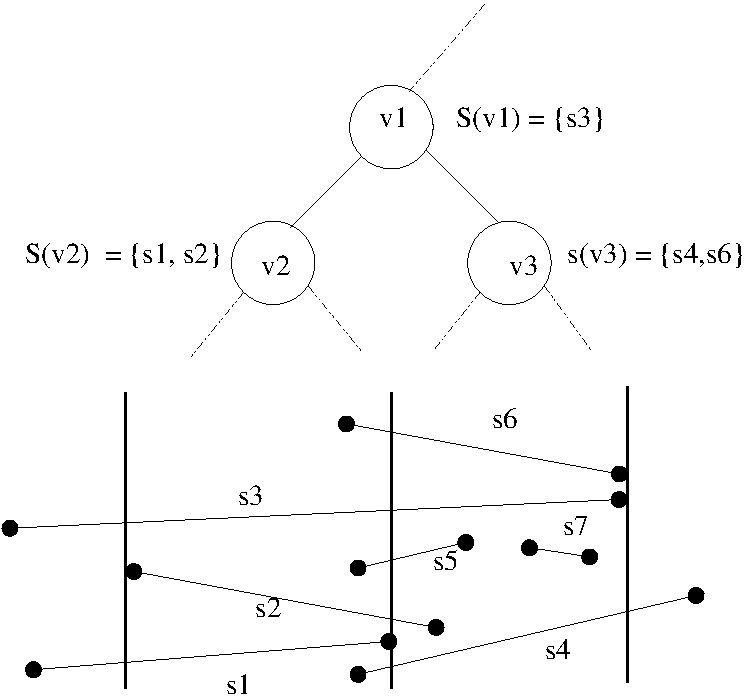
\includegraphics[scale=0.7]{images/segmentos_2d.pdf}
    \caption{Árvore de segmentos consultando 2D }
    \label{fig:my_label}
\end{figure}

\begin{algorithm}[h!]
    \caption{Recebe a raiz de uma árvore de segmentos $v$}
    \begin{algorithmic}[1]
        \Function{AtualizaEstruturasÁrvoreSegmentos}{$v$}
            \If{houver lista de segmentos $s$ em $v$}
                \State \Call{ConstroiÁrvoreAlcance}{$s_{y-intervalos}$}
            \EndIf
            \If {houver segmento em $filho_{esq}(v)$}
                \State \Call{AtualizaEstruturasArvoreSegmentos}{$v$}
            \EndIf
            \If{houver segmento em $filho_{dir}(v)$}
                \State \Call{AtualizaEstruturasArvoreSegmentos}{$v$}
            \EndIf
            
        \EndFunction
    \end{algorithmic}
\end{algorithm}

A consulta portanto terá uma adaptação. Ao invés de retornar todos os segmentos nos nós, realizaremos uma consulta dos segmentos nos nós quais destes estão dentro do intervalo de consulta $[y, y']$ na árvore $\rho$.

\begin{algorithm}[h!]
    \caption{Recebe a raiz de uma árvore de segmentos $v$, e um valor de consulta $q_x$. Retorna todos os segmentos que contêm o ponto $q_x$}
    \begin{algorithmic}[1]
        \Function{ConsultaArvoreSegmentos2D}{$v$, $q_x$}
            \State Reporte segmentos de \Call{Busca1DEmAlcance}{$\rho$, $[y, y']$}.
            \If{$v$ não é folha}
                \If{$q_x$ \in $Int(filho_{esq}(v))$}
                    \State \Call{ConsultaArvoreSegmentos2D}{$filho_{esq}(v)$, $q_x$}
                \Else
                    \State \Call{ConsultaArvoreSegmentos2D}{$filho_{dir}(v)$, $q_x$}
                \EndIf
            \EndIf
        \EndFunction
    \end{algorithmic}
\end{algorithm}

Por fim, para encontrar os segmentos inclinados em uma janela $J = [x, x'] \times [y, y']$, são necessárias duas árvores de segmento para cada eixo. E serão realizadas quatro consultas para cada aresta da janela. Detectando os segmentos que cruzam a janela e que não necessariamente tem um ponto dentro da janela. Enquanto que para detectar os pontos dentro da janela utilizamos uma árvore de alcance bidimensional e procuramos ao menos um ponto dentro da janela. 

\subsection{Resultados}
A fim de demonstrar o funcionamento da árvore desenvolvemos uma aplicação que constrói o mapa do Brasil com suas divisas intermunicipais, e conseguimos mostrar esse grande conjunto de pontos de forma eficiente.
Inicialmente lemos o arquivo que contem os pontos, criamos segmentos que os representam. Construímos uma árvore de alcance para detectarmos quais pontos estão dentro da janela, e uma árvore para identificarmos as bodas verticais da janela. Criamos um laço que se repete até sairmos da aplicação e para cada iteração consultamos ambas árvores e obtemos um conjunto de segmentos que podemos desenhar. Desenhamos cada um e o programa volta a iterar. Na Figura \ref{fig:execut1} (à direita) vemos a árvore de segmentos consultando os segmentos que cruzam a janela. Enquanto na Figura \ref{fig:execut1} (à esquerda) é a união das consultas da árvores de alcance para consultar os pontos extremos dos segmentos com o resultado da consulta na árvore de segmentos e quais segmentos cruzam a janela.

\begin{figure}[ht]
    \centering
    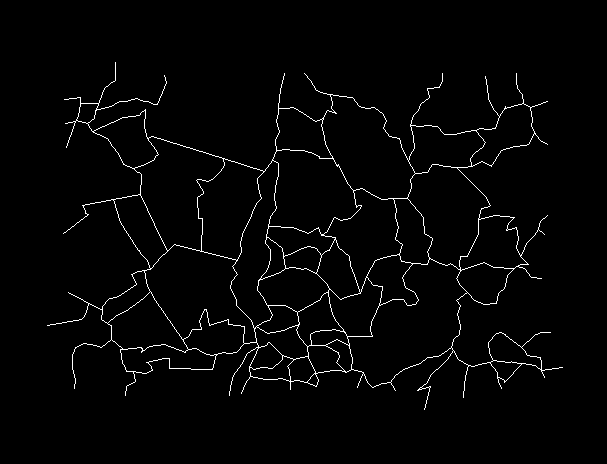
\includegraphics[scale=0.3]{images/Captura de tela de 2021-04-03 19-25-10.png}
    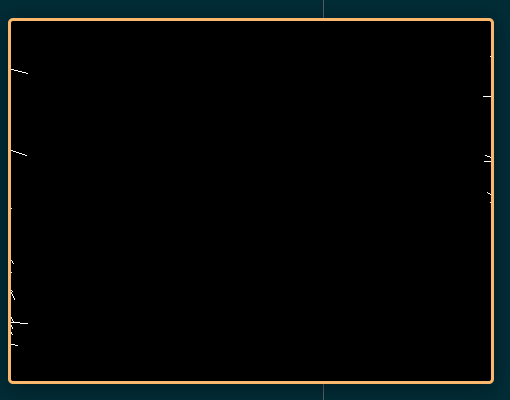
\includegraphics[scale=0.35]{images/Captura de tela de 2021-04-01 12-10-49.png}
    \caption{Janela de consulta do mapa do Brasil (à esquerda). Apenas a árvore de segmentos retornando os segmentos que cruzam as extremidades verticais da janela (à direita).}
    \label{fig:execut1}
\end{figure}

%\begin{figure}[ht!]
%    \centering
%    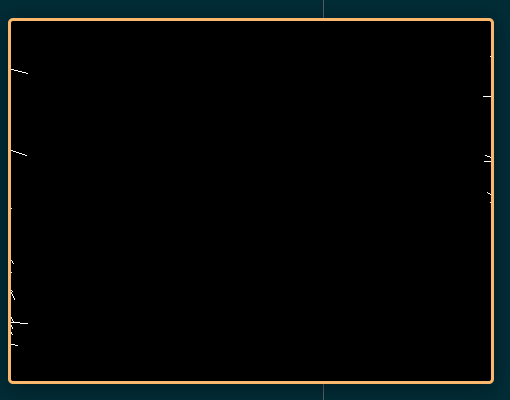
\includegraphics[scale=0.4]{images/Captura de tela de 2021-04-01 12-10-49.png}
%    \caption{Apenas a árvore de segmentos retornando os segmentos que cruzam as extremidades verticais da janela}
%    \label{fig:brazil_map_app}
%\end{figure}

%\clearpage